\begin{appendices}
\label{sec:Appendix}
\phantomsection

\myworries{Add Pictures of SEM-HyA\[ HyA1_2 and HyA1_3\]}


\section{Figures}
\label{appendix:fig}

\begin{figure}[hb!]
    \centering
    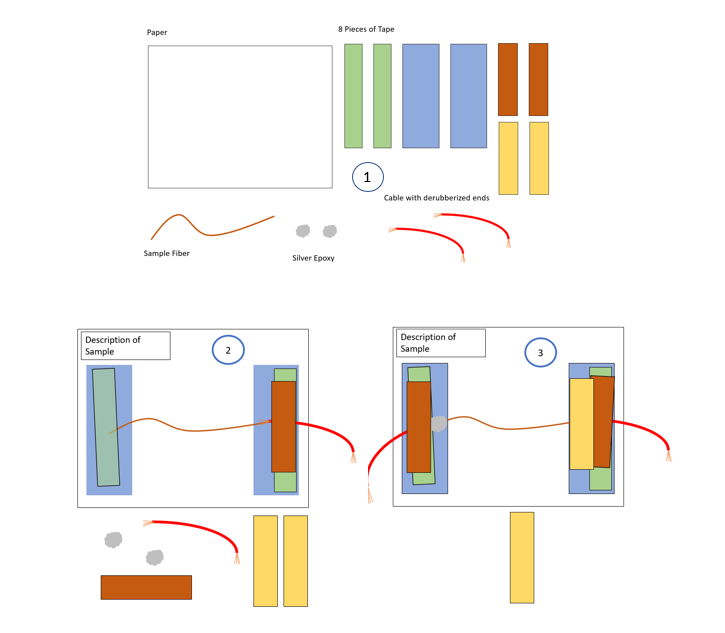
\includegraphics[width=.8\textwidth]{./pic/Meas_Prep_Together.PNG}
    \caption{Preparation for 
Strain-Resistance-Measurement}
    \label{fig:MeasPrep}
\end{figure}

\section{Pictures}

\myworries{Add Picture of bubbly sample}

\section{Protocols}
\label{App:Protocols}

\subsection{Sample Fabrication}

Prerequisites: \hfill\newline

\begin{multicols}{2}
	\begin{itemize}
		\item Gold concentration (\textit{c\textsubscript{gold}})
		\item Gold immersion time (\textit{t\textsubscript{gold}})
		\item Choice of reduction agent
		\item Reduction agent concentration (\textit{c\textsubscript{Red}})
		\item Reduction agent immersion time (\textit{t\textsubscript{Red}})
	\end{itemize}
\end{multicols}

\paragraph{Initial Protocol}

\begin{enumerate}
	\item Define which parameters are fixed and which are experimental parameters. Define range you want to investigate.
	
	\item Define concise naming concept, which allows every sample to be uniquely identified.
	
	\item Per sample reserve two petri dishes (PD) and label them in accordance with above mentioned concept. You might add the tag "Pre" and "Post" to existing description. (\textit{PDPre/PDPost}).
	
	\item Put 0.75ml of Gold Solution with \textit{c\textsubscript{gold}} in small, optimally non-translucent viol to account for the light-sensitivity of the gold salt (\textit{Viol}). One viol per sample you wish to investigate. Further decrease of translucency can be achieved by putting aluminium around viol.
	
	\item Put fiber in corresponding \textit{viol} and let immerse according to your defined \textit{t\textsubscript{gold}}.
	\item Take fiber out \textit{viol} and put in \textit{PDPre} to let dry. Note change in colour and/or structure. Experience shows that 30 minutes is sufficient.
	
	\item Gently pour 1ml of reduction agent solution with \textit{c\textsubscript{Red}} over fiber, while making sure the whole fiber is immersed. Note colour gradient in fiber and temporal resolution. Let immerse according to defined \textit{t\textsubscript{Red}}.
	
	\item After passing of time, transfer the fiber gently to \textit{PDPost}, where it will dry.
\end{enumerate}

\begin{center}
	This marks the end of the initial fiber fabrication.
\end{center}


\paragraph{Optimized Protocol} \hfill\newline

1. / 2. are identical to initial protocol.

\begin{enumerate}
	\setcounter{enumi}{2}
	
	\item Per sample reserve one petri dish (PD) and one glass slide (GS). Label them in accordance with above mentioned concept, whereas you might add the tag "Pre" to the PD and "Post" to GS description. (\textit{PDPre/GSPost}).
	
	\item Put 0.75ml of Gold Solution with \textit{c\textsubscript{gold}} in small, optimally non-translucent viol to account for the light-sensitivity of the gold salt (\textit{Viol}). One viol per sample you wish to investigate. Further decrease of translucency can be achieved by putting aluminum around viol.
	
	\item Put fiber in corresponding \textit{viol} and let immerse according to your defined \textit{t\textsubscript{gold}}.
	\item Take fiber out viol and put in \textit{PDPre} to let dry. Note change in color and/or structure. Experience shows that 30 minutes is sufficient.
	
	\item Gently pour 1ml of reduction agent solution over fiber, while making sure the whole fiber is immersed. Note color gradient in fiber and temporal resolution. Let immerse according to defined \textit{t\textsubscript{Red}}.
	
	\item After passing of time, transfer the fiber gently to \textit{GSPost}, where it will dry.
\end{enumerate}

\begin{center}
	This marks the end of the optimized fiber fabrication.
\end{center}

\subsection{Resistance Measurement}

\end{appendices}

